\chapter{Mise en œuvre}
\label{appendix:mise_en_oeuvre}

Le projet reprend un existant en C++, j'ai donc utilisé ce langage pour le développement.
Pour visualiser les solutions, j'ai également utilisé les langages HTML, JavaScript.

J'ai choisi d'écrire les solutions en JSON pour permettre les lires avec d'autres outils.


\section{Outils}

% Préciser ici Les outils et librairies utilisées (rapidement : les détails sur les versions exactes chose à savoir étant en annexe)

\subsection{Git}
Git est un outil de gestion de versions décentralisé et largement utilisé, je l'ai utilisé pour versionner mon code.
Il permet de garder l'historique des versions du projet et de comparer les versions.

\subsection{Github}
GitHub est une plateforme d'hébergement de dépôt Git qui propose également des outils pour gérer et suivre les tâche à réaliser et les demandes des utilisateurs.

\subsection{Visual studio}
Visual studio est un environnement de développement qui intègre les outils nécessaires au développement d'application en C++ et C\#.

\subsection{Tex Live}
Tex Live est une distribution latex qui est utilisé dans ce projet pour générer les rapports.

\subsection{Visual studio code}
Visual Studio Code est un éditeur de code modulaire et open-source créé par Microsoft.
Je l'ai utilisé pour : 
\begin{itemize}
    \item La rédaction des documents en Latex.
    \item Pour le développement d'un outil de visualisation de solution en HTML et Javascript.
    \item La lecture et mise en page des fichiers de solutions.
    \item La création de scripts PowerShell pour automatiser l'exécution de la recherche local avec différents paramètres.
\end{itemize}

\subsection{Doxygen}
Doxygen est l'outil qui a été utilisé pour générer la documentation du code du projet à partir de commentaires présents dans le code.


\section{Implémentations}

Le code du projet à été séparé en 4 parties :
- implémentation de la recherche locale
- implémentation de la méthode exacte avec CPLEX
- bibliothèque de fonctionnalités communes
- tests unitaires avec le Framework GTest

Durant le projet, j'ai également écrit un petit outil pour visualiser les données des solutions sous forme de diagramme de Gantt en HTML/javascript.

\subsection{Fonctionnalités communes}
Cette partie est la première que j'ai réalisé, car elle est nécessaire au développement des autres parties.

Je n'ai pas rencontré de problèmes particuliers lors de cette étapes mais elle a été plus longue que ce que j'avais prévue initialement.
Lors du développement de cette partie, j'ai également écrit les tests unitaires pour valider le fonctionnement de la bibliothèque.

\subsection{Utilisation du modèle mathématique}
Pour cette partie, j'ai implémenté le modèle mathématique que j'ai présenté précédemment.
J'ai rencontré successivement de nombreuses difficultés avec le solveurs CPLEX.
Après avoir résolu les nombreux problèmes de compilations et d'éditions des liens, j'ai obtenu une application qui donne des solutions invalides.
Je n'ai pas réussi à corriger ce problème, j'ai finalement dû passer à l'implémentation de la recherche local.

\subsection{Recherche locale}

Pour permettre de tester différents opérateurs de voisinage et méthode de sélection du meilleur voisin, 
ces opérateurs sont donnés  à l'instanciation de la recherche locale.

\subsubsection{Opérateurs de voisinage}
J'ai commencé par implémenter l'opérateur de voisinage par permutation des jobs dans l'ordre de production.
Par la suite j'ai implémenté un deuxième opérateur qui change la position des jobs dans l'ordre de production.

\subsubsection{Sélection du voisin}
Pour sélectionner le voisin à a choisir pour améliorer la solution, j'ai commencé par prendre le premier voisin qui est meilleur que la solution actuelle.
Par la suite, j'ai ajouté la stratégie qui consiste à sélectionner le meilleur voisin qui améliore la solution.

% \subsection{Déviations}
% J'ai pris du retard sur La méthode exacte donne des solutions invalides.

\subsection{Limites}

La résolution avec méthode exacte ne donne pas de solutions valides, je n'ai pas pu comparer les résultats des deux méthodes.
De plus sans la méthode exacte, je n'ai pas les meilleures solutions pour les instances testés,
j'ai donc comparé les résultats avec le meilleur résultat.

La génération de la fonction de coût par date de départ en livraison prend beaucoup de temps pour des lots de plus de 7 jobs,
lors des tests, il fallait 1 heure 30 pour résoudre un problème de 100 jobs avec des lots de 8 jobs.
Cette lenteur à rendu difficile l'évaluation de la recherche locale pour de grands lots.

% \subsection{Choix techniques}
% Les solutions sont exporté en suivant le forma JSON, 
% ce qui permet de les lire facilement, 
% aussi bien pour des utilisateur que pour des programmes.

\section{Performance}
La recherche locale s'exécute sur un seul thread, il serait possible de paralléliser une partie de la résolution.
La parallélisation n'a pas été mise en place dans ce projet dans le but de se concentrer sur les opérateurs.

\subsection{Analyse des résultats}

Pour la recherche local, j'ai comparé les résultats pour différents paramètres et opérateurs.
Pour faire les comparaisons, j'ai utilisé un script PowerShell pour tester automatiquement un grand nombre de combinaisons.
Le script extrait les données des solutions et les rassemble dans un fichier csv.
Les données du fichier CSV sont ensuite lut dans Excel et utilisé pour faire des graphiques.
\subsection{Operateur de voisinage}
Pour comparer les résultats sur plusieurs instances, j'ai calculé pour chaque solution, le rapport entre son score et le meilleur score obtenu pour l'instance.

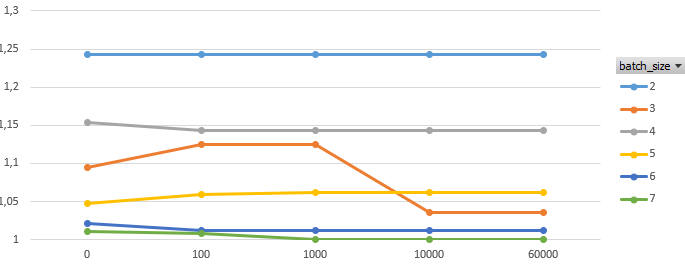
\includegraphics[width=\textwidth]{parts/mise_en_oeuvre/transposition}
Le graphique ci-dessus concerne l'opérateur de voisinage par permutations.
On peut voir l'évolution de la qualité de la solution en fonction de la durée de recherche locale (en millisecondes).
On remarque que le score n'évolue pas beaucoup avec augmentation de la durée, cela peut c'expliqué par le fait que les bâches soit de petites tailles, il y a donc un nombre limité de solutions à tester.

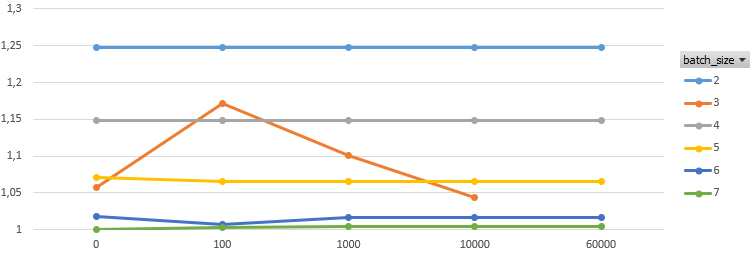
\includegraphics[width=\textwidth]{parts/mise_en_oeuvre/ordre}
Ce graphique concerne l'opérateur qui change les positions des jobs dans l'ordre de production.
De la même manière que pour l'opérateur précèdent, le résultat ne varie pas beaucoup avec la durée exécution.

Sur les 336 solutions regardées, le deuxième opérateur donne des résultats légèrement meilleurs.

\subsection{Sélection du voisin}

La méthode de sélection qui prend le meilleur voisin donne de meilleur résultats pour des temps de recherche très cours (moins d'une seconde).
Pour le reste, la méthode qui prend le premier voisin qui est meilleur donne de meilleurs résultats.
Ce résultat peut s'expliquer par le fait que les lots ne soit pas très grand et que la deuxième méthode soit très rapide.
La recherche locale explore donc plus de minimums locaux et peut plus facilement explorer toutes les solutions possibles.

